%Version 3.1 December 2024
% See section 11 of the User Manual for version history
%
%%%%%%%%%%%%%%%%%%%%%%%%%%%%%%%%%%%%%%%%%%%%%%%%%%%%%%%%%%%%%%%%%%%%%%
%% %%
%% Please do not use \input{...} to include other tex files. %%
%% Submit your LaTeX manuscript as one .tex document. %%
%% %%
%% All additional figures and files should be attached %%
%% separately and not embedded in the \TeX\ document itself. %%
%% %%
%%%%%%%%%%%%%%%%%%%%%%%%%%%%%%%%%%%%%%%%%%%%%%%%%%%%%%%%%%%%%%%%%%%%%

%%\documentclass[referee,sn-basic]{sn-jnl}% referee option is meant for double line spacing

%%=======================================================%%
%% to print line numbers in the margin use lineno option %%
%%=======================================================%%

%%\documentclass[lineno,pdflatex,sn-basic]{sn-jnl}% Basic Springer Nature Reference Style/Chemistry Reference Style

%%=========================================================================================%%
%% the documentclass is set to pdflatex as default. You can delete it if not appropriate. %%
%%=========================================================================================%%

%%\documentclass[sn-basic]{sn-jnl}% Basic Springer Nature Reference Style/Chemistry Reference Style

%%Note: the following reference styles support Namedate and Numbered referencing. By default the style follows the most common style. To switch between the options you can add or remove “Numbered” in the optional parenthesis. 
%%The option is available for: sn-basic.bst, sn-chicago.bst% 
 
%%\documentclass[pdflatex,sn-nature]{sn-jnl}% Style for submissions to Nature Portfolio journals
%%\documentclass[pdflatex,sn-basic]{sn-jnl}% Basic Springer Nature Reference Style/Chemistry Reference Style
% \documentclass[pdflatex,sn-mathphys-num]{sn-jnl}% Math and Physical Sciences Numbered Reference Style
\documentclass[pdflatex,sn-mathphys-ay]{sn-jnl}% Math and Physical Sciences Author Year Reference Style
%%\documentclass[pdflatex,sn-aps]{sn-jnl}% American Physical Society (APS) Reference Style
%%\documentclass[pdflatex,sn-vancouver-num]{sn-jnl}% Vancouver Numbered Reference Style
%%\documentclass[pdflatex,sn-vancouver-ay]{sn-jnl}% Vancouver Author Year Reference Style
%%\documentclass[pdflatex,sn-apa]{sn-jnl}% APA Reference Style
%%\documentclass[pdflatex,sn-chicago]{sn-jnl}% Chicago-based Humanities Reference Style

%%%% Standard Packages
%%<additional latex packages if required can be included here>

\usepackage{graphicx}%
\usepackage{multirow}%
\usepackage{amsmath,amssymb,amsfonts}%
\usepackage{amsthm}%
\usepackage{mathrsfs}%
\usepackage[title]{appendix}%
\usepackage[dvipsnames]{xcolor}
\usepackage{textcomp}%
\usepackage{manyfoot}%
\usepackage{booktabs}%
\usepackage{algorithm}%
\usepackage{algorithmicx}%
\usepackage{algpseudocode}%
\usepackage{listings}%
\usepackage{caption} % 
\renewcommand{\figureautorefname}{Fig.}
\renewcommand{\tableautorefname}{Table}
\newcommand{\Figref}[2][]{\hyperref[#2]{\figureautorefname~\ref*{#2}#1}}
\newcommand{\Tableref}[2][]{\hyperref[#2]{\tableautorefname~\ref*{#2}#1}}
%%%%

%%%%%=============================================================================%%%%
%%%% Remarks: This template is provided to aid authors with the preparation
%%%% of original research articles intended for submission to journals published 
%%%% by Springer Nature. The guidance has been prepared in partnership with 
%%%% production teams to conform to Springer Nature technical requirements. 
%%%% Editorial and presentation requirements differ among journal portfolios and 
%%%% research disciplines. You may find sections in this template are irrelevant 
%%%% to your work and are empowered to omit any such section if allowed by the 
%%%% journal you intend to submit to. The submission guidelines and policies 
%%%% of the journal take precedence. A detailed User Manual is available in the 
%%%% template package for technical guidance.
%%%%%=============================================================================%%%%

%% as per the requirement new theorem styles can be included as shown below
\theoremstyle{thmstyleone}%
\newtheorem{theorem}{Theorem}% meant for continuous numbers
%%\newtheorem{theorem}{Theorem}[section]% meant for sectionwise numbers
%% optional argument [theorem] produces theorem numbering sequence instead of independent numbers for Proposition
\newtheorem{proposition}[theorem]{Proposition}% 
%%\newtheorem{proposition}{Proposition}% to get separate numbers for theorem and proposition etc.

\theoremstyle{thmstyletwo}%
\newtheorem{example}{Example}%
\newtheorem{remark}{Remark}%

\theoremstyle{thmstylethree}%
\newtheorem{definition}{Definition}%

\raggedbottom
%%\unnumbered% uncomment this for unnumbered level heads

\begin{document}

%Modelling the synaptic interactions between two brainstem central pattern generators that coordinate breathing and swallowing
\title[Modeling synaptic interactions between mammalian breathing and swallowing central pattern generators]{Modeling synaptic interactions between mammalian breathing and swallowing central pattern generators}

%%=============================================================%%
%% GivenName	-> \fnm{Joergen W.}
%% Particle	-> \spfx{van der} -> surname prefix
%% FamilyName	-> \sur{Ploeg}
%% Suffix	-> \sfx{IV}
%% \author*[1,2]{\fnm{Joergen W.} \spfx{van der} \sur{Ploeg} 
%% \sfx{IV}}\email{iauthor@gmail.com}
%%=============================================================%%

\author*[1,3]{\fnm{Pavel} \sur{Tolmachev}}\email{pavel.tolmachev@princeton.edu}

\author[2]{\fnm{Rishi R. } \sur{Dhingra}}\email{rishi.dhingra@case.edu}
% \equalcont{These authors contributed equally to this work.}

\author[1]{\fnm{Jonathan H.} \sur{Manton}}\email{j.manton@ieee.org}
% \equalcont{These authors contributed equally to this work.}

\author[2]{\fnm{Mathias} \sur{Dutschmann}}\email{mathias.dutschmann@case.edu}
% \equalcont{These authors contributed equally to this work.}

\affil*[1]{\orgdiv{Department of Electrical and Electronic Engineering}, \orgname{University of Melbourne}, \orgaddress{\street{Grattan street 100}, \city{Melbourne}, \postcode{3010}, \state{Victoria}, \country{Australia}}}

\affil[2]{\orgname{Case Western Reserve University}, \orgaddress{\street{10900 Euclid Ave}, \city{Cleveland}, \postcode{44106}, \state{Ohio}, \country{USA}}}

\affil*[3]{\orgdiv{Princeton Neuroscience Institute}, \orgname{Princeton University}, \orgaddress{\street{Washington Road}, \city{Princeton}, \postcode{08540}, \state{New Jersey}, \country{USA}}}

%%==================================%%
%% Sample for unstructured abstract %%
%%==================================%%

\abstract{Breathing and swallowing are tightly coupled motor behaviors whose execution depends on the coordinated activity of two brainstem central pattern generators (R-CPG, Sw-CPG). We present a mechanistic neural network model that captures this coordination. The model was built by incrementally expanding the synaptic connectivity of R-CPG and Sw-CPG modules, each composed of neuronal population nodes whose dynamics incorporate firing rate adaptation. The rhythmogenic cores of both CPGs are implemented as half-center oscillators operating independently. In agreement with accompanying experimental recordings from an \textit{in situ} perfused brainstem preparation, a simulated 10~s sensory drive to the superior laryngeal nerve (SLN) reliably elicits fictive sequential swallowing bursts accompanied by glottal closure and suppression of inspiratory activity. Short SLN stimuli (100~ms) produce isolated single swallows that reset the phase of the respiratory oscillator. Phase space analysis of the model dynamics offers additional insight into this SLN-evoked respiratory phase resetting. Consistent with prior experimental observations, simulated pontine lesions reproduce apneusis and abolish swallowing-related glottal closure during sequential swallowing. Systematic perturbation of synaptic weights across specific network pathways identifies vulnerable connections whose weakening recapitulates clinically relevant breathing--swallowing disorders, including aspiration. The model thereby generates mechanistic predictions that may inform the design of therapeutic interventions for conditions characterized by impaired breathing--swallowing coordination.}
\keywords{postinspiration, dorsal swallowing group, pontine respiratory group, pre-Bötzinger complex, digestion, brainstem, computational model}
%%\pacs[JEL Classification]{D8, H51}
%%\pacs[MSC Classification]{35A01, 65L10, 65L12, 65L20, 65L70}

\maketitle

\section{Introduction}\label{sec: introduction}
Swallowing and breathing are two fundamental motor behaviors whose coordination is essential for survival. Unlike breathing, which proceeds autonomously and tolerates only brief interruption before hypoxic injury ensues, swallowing is triggered conditionally---either through sensory afference carried predominantly by the superior laryngeal nerves \citep{miller1974anatomical, jafari2003sensory, hashimoto2019activity, sang2001swallowing} or through descending volitional commands \citep{mosier2001parallel,ludlow2015central, wei2024cortical, trevizan2024neuroanatomical}. Both air and ingested material share the oropharyngeal passage, and a coordinated sequence of oropharyngeal muscle contractions is required to propel food and liquids from the mouth to the esophagus and onwards to the stomach \citep{miller1986neurophysiological, sejdic2018computational, allen2012deglutition, jean2001brain}. A substantial subset of these muscles also participates in the breath-by-breath regulation of upper airway patency \citep{bartlett1989respiratory, dutschmann2002glycinergic, dutschmann2014physiological, bolser2013central, bautista2014generation}. Among them, the laryngeal adductors---which draw the vocal folds toward the midline---are active in both contexts. During expiration, graded adduction resists outward airflow and thereby regulates expiratory duration and effort \citep{harding1984perinatal, bartlett2011upper, dutschmann2002influence, dutschmann2002glycinergic, dutschmann2006kolliker, dutschmann2014physiological}, while complete adductor-driven glottic occlusion during swallowing shields the subglottic airway from aspiration, a requirement that is particularly stringent during repetitive sequential swallowing \citep{bolser2006neurogenesis,bolser2015role, dutschmann2014physiological}. 

The motor programs for respiration and swallowing are produced by anatomically overlapping networks---the respiratory and swallowing central pattern generators (R-CPG, Sw-CPG)---distributed throughout the brainstem \citep{bianchi2009brainstem}. The R-CPG occupies bilateral ponto-medullary columns of respiratory neurons \citep{alheid2004pontine}, yet accumulating evidence indicates that the characteristic eupneic three-phase motor output---comprising inspiration, postinspiration, and late expiration---depends on synaptic recruitment of the dorsal respiratory group as well \citep{berger1977dorsal, hilaire1990functional, dhingra2019excitation, dhingra2019increasing, dhingra2020volumetric}. This dorsal respiratory group substantially overlaps with the dorsal swallowing group of the Sw-CPG, housed within the nucleus of the solitary tract (NTS) \citep{car1979inputs, kalia1980brain, kessler1985identification, jean2001brain} of the caudal medulla. A second Sw-CPG compartment, the ventral swallowing group, is positioned dorsomedial to the nucleus ambiguus \citep{kessler1985identification, ezure1993location, sugiyama2011axonal, fuse2019effects, huff2023role, toor2019neurons} and may coincide with the postinspiratory complex (PiCo) \citep{toor2019neurons, pitts2021evidence, huff2023role} of the rostral medullary reticular formation. In addition, pontine K\"olliker-Fuse neurons have been shown to gate swallow-related sensory transmission and to contribute directly to breathing--swallowing coordination \citep{bautista2014ponto, takemura2022effect}. Taken together, swallowing- and breathing-related neurons are broadly distributed across the ponto-medullary neuraxis. Nevertheless, the specific synaptic pathways linking Sw-CPG and R-CPG populations---and thereby ensuring the precise temporal coupling of the two behaviors---remain incompletely resolved, largely because the functional neuroanatomy of the short- and long-range connections bridging these two CPGs has yet to be fully characterized.

The computational neuroscience of breathing has been dominated for three decades by Hodgkin--Huxley-type models that dissect the synaptic underpinnings of respiratory rhythmogenesis and the three-phase motor pattern \citep{rybak1997modeling, rybak2004modeling, smith2007spatial, rubin2009multiple, molkov2013control, molkov2014closed, molkov2017computational, lindsey2012computational}. Network responses to peripheral sensory challenges---including the Hering--Breuer inflation reflex \citep{molkov2013control} and hypoxia or hypercapnia \citep{molkov2014closed}---have been captured in such frameworks, yet to our knowledge only a single study has addressed the coupling of two distinct motor CPGs, specifically in the context of respiratory--locomotor entrainment \citep{potts2005respiratory}. Conceptual circuit diagrams for breathing--swallowing coordination have appeared \citep{bolser2013central, pitts2013coordination}, but a quantitative, mechanistic computational model has not yet been established. 

Here we extend established R-CPG models \citep{smith1991pre, rybak2004modeling, rubin2009multiple} by embedding a putative synaptic architecture that enables the coordination of breathing and swallowing within a single unified framework. Both the R-CPG and Sw-CPG are formulated as half-center oscillators (HCOs) cast as Matsuoka neural oscillators \citep{matsuoka2011analysis} with streamlined population-level dynamics, deliberately emphasizing inter-population connectivity over cell-intrinsic biophysics. The model is compared to experimental recordings of SLN-evoked swallowing from an \textit{in situ} perfused brainstem preparation. Under simulated 10~s SLN drive the model reproduces sequential swallowing with simultaneous glottal closure, while a brief 100~ms stimulus reliably triggers a solitary swallow that perturbs the respiratory cycle in a timing-dependent manner. This perturbation is fully described by a phase-resetting curve (PRC) whose profile is in qualitative agreement with prior experimental data \citep{oku1992phase}. Systematic variation of synaptic weights further reveals vulnerable circuit loci whose disruption mirrors clinically relevant breathing--swallowing pathologies.

\section{Methods}\label{Methods}

\subsection{Experimental data acquisition}
All experimental procedures received ethical approval from the Animal Ethics Committee of the Florey Department of Neuroscience \& Mental Health, University of Melbourne, Melbourne, Australia (17-077FINMH), and were carried out in full compliance with institutional animal welfare regulations.
Juvenile Sprague–Dawley rats of both sexes (postnatal days 17–21) were used in the \textit{in situ} arterially perfused brainstem preparation, following established protocols \citep{paton1996working, dutschmann2000respiratory}. Animals were deeply anesthetized with isoflurane (2–5\%) and, once a surgical plane of anesthesia was confirmed, transected subdiaphragmatically before rapid transfer to an ice-cold bath of artificial cerebrospinal fluid (aCSF; in mM: 125 [$\text{NaCl}$], 3 [KCl], 1.25 [$\text{KH}_2\text{PO}_4$], 1.25 [$\text{MgSO}_4$], 25 [$\text{NaH}\text{CO}_3$], 2.5 [$\text{CaCl}_2$], 10  D-glucose 1.25\% Ficoll---an oncotic agent; Sigma‒Aldrich, Steinheim, Germany) for decerebration. Following removal of the heart and lungs, the phrenic nerve was dissected free for recording, the descending aorta was exposed for cannulation, the cerebellum was aspirated, and both the vagus and superior laryngeal nerves were isolated for recording and stimulation, respectively. \\
The brainstem was then transferred to a recording chamber, the aorta cannulated with a double-lumen catheter, and reperfusion commenced with carbogenated (95\%/5\% pO2/pCO2), warmed (31\,°C) aCSF driven by a peristaltic pump (Watson-Marlow). Phrenic and vagal nerves were drawn onto suction electrodes to capture fictive respiratory and swallowing discharge. Nerve potentials were amplified ($400\times$), band-pass filtered (1–7500~Hz), sampled at 30~kHz through a 16-channel differential headstage (Intan RHD2216), and archived with an Open Ephys acquisition system (Rev. 2; \citet{siegle2017open}). Apneustic activity typically resumed within minutes; a bolus of sodium cyanide (NaCN; 0.1~mL, 0.1\% w/v) was then injected to provide chemosensory drive that converted the apneustic discharge into a stable eupneic three-phase respiratory motor pattern, after which perfusion flow was fine-tuned to maintain rhythmic stability.

To evoke swallowing, the superior laryngeal nerve (SLN) was stimulated electrically. The current threshold for triggering swallows was first identified using 10~s trains (20~Hz, 0.1~ms pulse width) at amplitudes stepped from 10 to 80~µA; sequential swallowing was then assessed at twice this threshold.
To map the SLN phase-resetting curve, single swallows ($n = 100$) were elicited at pseudorandom inter-stimulus intervals of 20–25~s (20~Hz, 250~ms burst duration, 0.1~ms pulse width, $2\times$ threshold current), ensuring coverage of all respiratory cycle phases.

\subsection{Experimental data analysis}
Signal processing of the vagus and phrenic nerve recordings was carried out in Python using routines from the SciPy library \citep{2020SciPy-NMeth}. Each trace was first mean-centred, then bandpass-filtered with a second-order Butterworth filter (\texttt{signal.butter}, passbands: 300~Hz--3~kHz). To prevent phase distortion, every filtering step employed zero-phase forward--backward application (\texttt{signal.filtfilt}). Artefacts from SLN stimulus pulses were removed by linearly interpolating across each stimulus epoch, eliminating the immediate transient deflections without affecting surrounding signal. The absolute value of the resulting signal was taken, and the envelope was further smoothed with a second-order low-pass Butterworth filter (12~Hz cut-off); the processed vagal trace closely resembled a respiratory airflow waveform, and both phrenic and vagal signals became well-suited for downstream analysis. The signals were then decimated by a cumulative factor of 100 through two successive calls to \texttt{signal.decimate} (factor of 10 per step, with anti-aliasing filtering applied at each stage), yielding a final sampling rate of 300~Hz.

The PRC quantifies the dependence of respiratory cycle phase shift on the timing of a brief SLN stimulus within the cycle. To construct it, the continuous recording was segmented into epochs each containing exactly one SLN stimulation event (\Figref[A]{fig: PRC_comparison}). Within each epoch, the phrenic nerve activity (PNA) was additionally low-pass filtered (\texttt{signal.butter}, cut-off frequency = 1~Hz) to isolate the fundamental respiratory oscillation (0.2--1~Hz). The instantaneous phase (protophase) was estimated via the Hilbert transform \citep{kralemann2008phase} following subtraction of the analytic signal mean. The oscillation frequency $\omega_0$ was obtained from a linear fit to the pre-stimulus protophase, and a refined phase $\phi$ was subsequently computed following \citep{kralemann2008phase}.
Pre- and post-stimulus phase trajectories were each described by linear fits $\phi_b = \omega_0 t + b_1$ and $\phi_a = \omega_0 t + b_2$, with $\omega_0$ held fixed during optimization (\texttt{optimize.minimize}); the phase shift was then computed as $\Delta \phi = (b_1 - b_2)$ (\Figref[A]{fig: PRC_comparison}).

\subsection{Model parameters}
Previous studies that modeled R-CPG function incorporated Hodgkin-Huxley style biophysical properties of respiratory neurons \citep{smith2007spatial, rubin2009multiple, molkov2013control, molkov2014closed, molkov2017computational}. However, such models are prone to overfitting \citep{del2018breathing}. Instead of using Hodgkin-Huxley style description, we model neuronal populations with simpler equations underlying the Matsuoka neural oscillator \citep{matsuoka2011analysis}; which allows the R-CPG and Sw-CPG to function with a reduced parameter set, focusing on their interaction:
\begin{align*}
 \tau_v \frac{dv}{dt} &= -\alpha v - m + (\text{drive} - b)+\text{input} \\
 \tau_m \frac{dm}{dt} &= s(v) - m, 
\end{align*}
where $s(v) = 1/(1+e^{-\lambda v} )$ - activity level of a population, $s(v) \in (0,1)$.
In these equations, the dimensionless variable v is analogous to the average membrane potential of a whole neural population. The variable $m$ mediates the firing rate (spike frequency) adaptation and acts on a much slower timescale than the variable $v$. To account for the correct timescale of the dynamics and the excitability of the neuronal populations, we use $\alpha=1$, $b=0.2$, $\tau_v=2$~ms, $\lambda=30$. The parameter $\tau_m$, which controls the timescale of firing rate adaptation, has distinct values for the different neuronal populations (discussed later), and the details are summarized in \Tableref{tbl: intrinsic_params}. The parameters are chosen manually to match the timescale of respiratory phase durations (inspiration, postinspiration, late expiration) of experimental recordings.
The term `input' in the equations incorporates synaptic input from the other nodes of the neuronal populations of the R-CPG or Sw-CPG, as well as the sensory input from the SLN (applicable only to the Sensory Relay neurons, see later). The synaptic input to population j is modeled by the following equation:
\begin{align*}
 \text{input}_j = \sum_{i \in C}^N w_{ij} s(v_i) +\text{stimulus}_j 
\end{align*}
Where $C$ is the set of neural nodes projecting to the $j^{th}$ neuron.
The stimulus term represents a square pulse input applied to `Sensory Relay' neurons during SLN stimulation.
The connectivity parameters $w_{ij}$ between the nodes are manually adjusted to reproduce realistic swallowing and breathing interactions. The gradual development of the model (\Figref[]{fig: model_sequence}) allowed for adjusting connectivity parameters step by step, and the connectivity of a simpler model served as a reference point for the connectivity of a subsequent model. The resulting model (\Figref[]{fig: complete_model}) is used for simulation of the phrenic and vagus nerve activities. The baseline level of activity of an isolated neuronal population is controlled by the parameter `drive' which physiologically corresponds to the tonic excitatory drive from the other brain regions.

\subsection{Sequential development of the model connectivity}
Using the equations for the neuronal populations defined above, we developed the network connectivity in 4 successive steps (\Figref[]{fig: model_sequence}). 
The initial model (Model 1; \Figref[A]{fig: model_sequence}, \Figref[]{fig: model1_dynamics}) established the basic connectivity: a half-center oscillator in the R-CPG generates biphasic respiratory activity (inspiration (`I') and expiration (`E')), and a conditionally active half-center oscillator for the Sw-CPG (`$\text{Sw}_1$', `$\text{Sw}_2$' populations) produces a sequence of rhythmic swallows in response to a simulated 10~s sensory input from the SLN. The premotor `$\text{Sw}_1$' neurons in Sw-CPG contribute to the vagus nerve discharge. The ‘Sensory Relay’ neurons, whose activity indicates the presence of the sensory stimulus, are comprised of excitatory and inhibitory neuronal populations. The excitatory `Sensory Relay' subpopulation provides drive for the Sw-CPG, while the inhibitory subpopulation suppresses the activity of the inspiratory populations in the R-CPG during ongoing swallowing. In the initial model, a 10~s sensory input from the SLN (\Figref[]{fig: model1_dynamics}) evokes the swallowing related bursts of activity in the vagus nerve output for the larynx that resembles the pharyngeal phase of swallowing (for details see \citep{jean2001brain, bautista2014ponto, lang2009brain}). The large value of firing rate adaptation time constant of the `Sensory Relay' neurons is responsible for a slowly declining frequency of the sequential swallows. The simulated SLN stimulation effectively suppresses inspiratory activity during the 10~s period of swallowing.
In the next model iteration (Model 2, \Figref[B]{fig: model_sequence}), the R-CPG was separated into medullary and pontine compartments to reflect experimental findings that pontine neurons control Sw-CPG gating \citep{bautista2014ponto}. An excitatory postinspiratory population was also added to the pons to account for the tonic postinspiratory activity mediating glottal closure during sequential swallowing \citep{bautista2014ponto}.

The next stage of the model evolution (Model 3, \Figref[C]{fig: model_sequence}) incorporates an additional expiratory neuronal population to the R-CPG (`Late-E') to generate a three-phase respiratory motor pattern, as the hallmark of previous R-CPG model simulations \citep{smith1991pre, rybak1997modeling, rybak2004modeling, rubin2009multiple, molkov2013control, molkov2014closed, molkov2017computational}. The core of the R-CPG is thus modelled as a ring of three mutually inhibiting populations of inspiratory (`Insp'), postinspiratory (`Post-I') and late-expiratory population (`Late-E', active during the second half of the expiration, E2).
In the final model (Model 4; \Figref[D]{fig: model_sequence}) we incorporate an additional premotor `Ramp-I' population of neurons to account for a eupneic respiratory motor activity that requires a ramping discharge pattern of the simulated phrenic nerve activity (PNA) and vagus nerve activity (VNA) \citep{john2003defining, harris2017different}. No intrinsic neural mechanisms have been found to cause a rapid increase in firing rate followed by a sudden stop in activity; therefore, this discharge pattern was hypothesized to result from inhibitory (mainly local) connections \citep{harris2017different}. 

In the final model, the outputs of PNA and VNA were simulated as weighted sum of the activities of `Ramp-I', `Pontine Post-I', and `$\text{Sw}_1$' populations. The connectivity parameters between populations are listed in \Tableref{tbl: connectivity_params}.
We implemented multiple sources of tonic drives for the R-CPG and Sw-CPG neuronal populations in the final model: the `Arousal drive', the `Descending pontine drive' for the medullary respiratory circuit, and the `Chemo-drive' (\Figref[]{fig: complete_model}). In accordance with experimental findings \citep{sato2011sleep, sato2016deglutition}, the `Arousal drive' controls the excitability of the Sw-CPG. The `Descending pontine drive' predominantly regulates the excitability of `post-I' neurons in the medullary compartment of the R-CPG \citep{dutschmann2006kolliker, rybak2004modeling, rybak2004modelling}. Lastly, the `Chemo-drive' projects to `late-E' populations but also provides excitation to the medullary inspiratory neurons. The specific settings for the tonic drives are summarized in \Tableref{tbl: drives}.

The timescale of firing rate adaptation $\tau_m$ is set to be smaller for the modelled populations in Sw-CPG compared to the neuronal populations of the medullary R-CPG. Such difference in the intrinsic properties is introduced to account for the generation of a physiologically plausible number of swallows during simulated 10~s SLN stimulation. Additionally, we modelled the `Sensory Relay' and the `pontine post-I' populations to have much lower firing rate adaptation than the medullary R-CPG populations, to account for the slower timescale of a decrementing swallowing-related glottal closure activity during 10~s SLN stimulation. The intrinsic properties of the neural groups are summarized in \Tableref{tbl: intrinsic_params}. 

\subsection{Modeling of a single swallow in response to short SLN stimulation in the Sw-CPG}
In physiological experiments using the perfused brainstem preparation, a short (100-250~ms) stimulation of the SLN evoked a single swallow after the termination of the stimulus, which caused modulation of the respiratory cycle duration (See Results). To account for these experimental findings, `Sensory Relay' neurons excite both `$\text{Sw}_1$' and `$\text{Sw}_2$' populations, which comprise a swallowing half-center oscillator. During eupneic breathing, the `$\text{Sw}_2$' neurons receive more arousal drive than the `$\text{Sw}_1$' neurons, leading to the inhibition of the `$\text{Sw}_1$' premotor population. In our model, a 100~ms SLN stimulation provides additional excitation to both `$\text{Sw}_1$' and `$\text{Sw}_2$' populations; however, the `$\text{Sw}_2$' neurons outcompete the `$\text{Sw}_1$' population, and, at the onset of the stimulus, the `$\text{Sw}_2$' neurons further inhibit the ‘$\text{Sw}_1$’ population. After cessation of the 100~ms SLN stimulation, the `$\text{Sw}_1$' premotor neurons exhibit a post-inhibitory rebound, escaping the `$\text{Sw}_2$' inhibition, thus producing a solitary swallowing motor burst. This mechanism is further analyzed using a phase space analysis (See Results).

\section{Results}\label{sec: results}
The present computational model of breathing-swallowing interaction depicts each CPG as a half-center oscillator, described by simplified equations adapted from the Matsuoka neural oscillator. In accordance with published data \citep{fuse2025spatio}, a separate neuron population relays sensory inputs from the SLN to the swallowing network. The respiratory half-center oscillator underlies inspiratory-expiratory phase oscillations, while the swallowing oscillator generates stimulus-dependent sequential pharyngeal swallowing activity (Model 1, \Figref[A]{fig: model_sequence}; \Figref[]{fig: model1_dynamics}). Later, we progressively introduce additional neuronal populations (\Figref[B,C,D]{fig: model_sequence}) to account for experimental data (both previously published, and obtained presently). The final model (\Figref[]{fig: complete_model}) reproduces the eupneic three-phase motor pattern of respiration characterized by incrementing phrenic nerve activity (PNA) and decrementing postinspiratory activity in the vagal nerve, as shown in previously published models \citep{rybak2004modeling, smith2007spatial}.

Simulation of 10~s synaptic input from the SLN forces the two reciprocally inhibiting swallowing populations to compete and oscillate between active (`$\text{Sw}_1$') and silent phases (`$\text{Sw}_2$') resembling the activity during the pharyngeal phase of swallowing \citep{hashimoto2019activity, bautista2014generation, kinoshita2021influences, jean2001brain}. `$\text{Sw}_1$' neurons represent an excitatory premotor subpopulation that drives laryngeal motor output during swallowing, while `$\text{Sw}_2$' interneurons provide no output to upper airway muscles. In parallel, `Sensory Relay' neurons inhibit inspiratory (`Insp') and late expiratory (`Late-E') neuronal populations of the R-CPG and consequently arrest the three-phase respiratory cycle in the postinspiratory phase (`Post-I'). In addition, excitatory `Sensory Relay' neurons project to the `Pontine Post-I' neural population, which excites the medullary `Post-I' neurons and drives the vagal motor output to the larynx to mediate the protective swallowing-related glottal closure during sequential swallowing \citep{bautista2014ponto}. Comparison of model performance with experimental data shows that 10~s electrical stimulation of the SLN elicits 5 to 14 swallows, while simulated 10~s SLN input in the model triggers a comparable number of 5 to 7 swallows (\Figref[]{fig: swallowing_and_eupneic_breathing}). The model also qualitatively reproduces the experimental data from randomly timed short SLN stimulations in the perfused brainstem preparation: similar to the experimental data, the simulated 100~ms stimulus evokes a single swallowing-related burst, which causes timing-dependent modulation of the respiratory cycle length (\citet{lewis1990effects, oku1992phase}, see below; \Figref[A]{fig: PRC_comparison}).

\subsection{Model validation: phase response curve}
Newly acquired and previously reported experimental data obtained in a perfused brainstem preparation of a rat \citep{paton1996working, paton2022advancing} showed that the application of a short train (20~Hz, 250~ms) electrical stimulation of the SLN caused either a decrease or an increase in the respiratory cycle length depending on the timing of the stimulus during the breathing cycle (\Figref[A]{fig: PRC_comparison}). For instance, when the stimulation of the SLN was delivered during the inspiratory phase, the stimulus caused short-latency termination of ongoing phrenic nerve activity, while initiating a solitary swallow. The subsequent respiratory cycle was shortened due to a decrease in the expiratory phase duration \citep{horton2018central, oku1992phase}. Short SLN stimulation applied during the late expiratory phase also evoked a solitary swallow; however, in this case the stimulation increased the expiratory phase duration and lengthened the overall respiratory cycle length. The effects of short SLN stimulation are summarized by a phase response curve (PRC), which has become a standard tool for the analysis of oscillatory dynamical systems \citep{galan2005efficient, izhikevich2007dynamical}. Although the PRC estimated from experimental recordings exhibited a low signal-to-noise ratio, its overall shape qualitatively matched the PRC obtained from the simulation of the computational model (\Figref[B,C]{fig: PRC_comparison}). 

\subsection{Phase space analysis of the Sw-CPG: transient dynamics of the swallowing half-center oscillator in response to a short SLN stimulation}
A short stimulation of the superior laryngeal nerve triggers a swallow that either delays or advances the phase of the respiratory rhythm, depending on the timing of SLN stimulation \citep{lewis1990effects, oku1992phase}. The mechanisms underlying the generation of a short-latency single swallow in response to short SLN stimulation could depend on the ion channel composition (e.g. HCN, BK and SK channels, \citep{molineux2008ionic}) of SW-CPG neuron populations. Rather than focusing on the kinetics of individual ion channels, we instead modeled the generation of the short-latency swallowing response at a higher level of dynamical abstraction, capturing post-inhibitory rebound of the premotor neurons ($\text{Sw}_1$) using minimal dynamical-system complexity. We implemented an asymmetric tonic excitatory drive (Arousal drive') for the $\text{Sw}_1$' and $\text{Sw}_2$' neural populations, along with descending inhibition of the $\text{Sw}_1$' population from the pontine swallowing gate (sw-gate control'). Together, these inputs establish baseline excitation levels of $0.17$ for $\text{Sw}_1$' and $0.35$ for $\text{Sw}_2$'. As a result, during SLN stimulation, the $\text{Sw}_1$' premotor neurons are less excitable than the $\text{Sw}_2$' population, and the oscillation begins with the motor-silent phase ($\text{Sw}_2$' active). Since $\text{Sw}_1$' neurons mediate the swallowing-related vagal motor output, this configuration accounts for the physiologically observed delay in swallow initiation following short SLN stimulation (visible in the vagus nerve activity, VNA), as the response initially recruits the $\text{Sw}_2$' population.

To see this dynamical mechanism in action, we further analyzed the effect of excitatory inputs from the `Sensory Relay' neuronal population on the Sw-CPG using dynamical system theory. \Figref[]{fig: PIR_mechanism} illustrates two different scenarios that discriminate the occurrence of a short-latency single swallow in response to a short SLN stimulation: in the first scenario, a short-latency swallowing response is observed after the stimulation, resembling the swallowing response in the experimental conditions; whereas in the second scenario, the swallowing response is immediate and is concurrent with the stimulus, being unphysiological. 
Both scenarios differ only in the strengths of the sensory input to the swallowing populations. In the first scenario (\Figref[A]{fig: PIR_mechanism}, short-latency single swallow), the strengths of the sensory input to the `$\text{Sw}_1$' and `$\text{Sw}_2$' neurons required a setting of $0.12$ and $0.07$, respectively. In scenario 2, a small increase of the input strength to the `$\text{Sw}_1$' population up to $0.19$ prevents the occurrence of the normal swallowing response to the short SLN stimulation (\Figref[C]{fig: PIR_mechanism}, the swallowing response is concurrent with the SLN stimulation). 

To study the difference between these scenarios we performed a phase space analysis of the dynamics of the Sw-CPG. The evolution timescales of $v$-variables and $m$-variables differ by three orders of magnitude. Therefore, the whole system can be subdivided into fast and slow subsystems. During the evolution, the $v_1$ and $v_2$ variables are almost functionally dependent, $v_1 \approx f(v_2)$; therefore, one of the fast variables could be eliminated from the analysis, and the dynamics are effectively described in the three-dimensional phase space.
For each fixed pair of slow $m$-variables $(m_1,m_2)$, we calculated fixed points of the fast subsystem dynamics $(v_1^*,v_2^*)$, which form a surface. The equilibrium surface in $(m_1,m_2,v_1)$-space forms a cusp (\Figref[B]{fig: PIR_mechanism}), a region where the surface folds back on itself so that multiple values of one variable correspond to the same parameter set. This S-shaped structure implies the presence of two stable equilibria on the outer sheets and one unstable equilibrium on the middle sheet.
In the global equilibrium (Point 1 in \Figref[A,B]{fig: PIR_mechanism}), the system stays on the lower sheet of the equilibrium surface, albeit close to the cusp (lower knee of `S', just before the cusp). The location of the global equilibrium corresponds to the quiescent `$\text{Sw}_1$’ neurons, since the value $s(v_1)$ is close to zero, although the system is readily excitable.

In the first scenario, the stimulus drives the system away from the lower sheet of the equilibrium surface into the region of the overhanging upper sheet. The state then jumps `vertically' (along $v_1$ axis) to the upper sheet, from which it gradually slides down until it reaches the boundary of the cusp. While on the upper sheet, the variable $v_1$---representing activity of the premotor $\text{Sw}_1$ neurons---remains elevated, indicating a solitary swallowing response. Once the state reaches the cusp, it abruptly falls back to the lower sheet, corresponding to termination of the solitary swallow (\Figref[A,B]{fig: PIR_mechanism}, points 1-2-3-4). In contrast, in the second scenario, the stimulus shifts the system away from the upper sheet, and once the input ceases, the state immediately relaxes back to the lower sheet (where $\text{Sw}_1$ remains quiescent), producing no transient post-stimulus activity (\Figref[C,D]{fig: PIR_mechanism}, points 1-2-3).
In the model, the swallowing response is therefore determined by the cusp-like shape of the equilibrium surface of the fast subsystem, implementing post-inhibitory rebound of the premotor swallowing population.

\subsection{Model validation: silencing of pontine neuronal populations.}
To test whether the proposed ponto-medullary connectivity captures known physiological dependencies, we simulated inhibition of the pontine compartment (\Figref[]{fig: eupn_vs_apn}).
Previously published data have shown that pharmacological inhibition of the pontine compartment of the R-CPG triggered apneusis (prolonged inspiratory phase and absence of postinspiratory motor discharge in VNA, \cite{dutschmann2006kolliker}). Inhibition of the pontine populations of the R-CPG had modest effects on SLN-evoked sequential swallowing motor pattern \citep{takemura2022effect} but abolished protective glottal closure during physiologically evoked swallowing \citep{bautista2014ponto}. The latter study also reported that pharmacological inhibition of the pons caused spontaneous swallowing activity in the absence of sensory input. The results of simulated inhibition of the pons are depicted in (\Figref[B]{fig: eupn_vs_apn}) and the motor output is compared to the simulated eupneic motor activity (\Figref[A]{fig: eupn_vs_apn}). In line with experimental data, the simulation of pontine inhibition is characterized by an increase in inspiratory phase duration ($T_i$ from $0.41 \pm 0.05$ to $1.29 \pm 0.05$~s) and expiratory phase duration ($T_e$ from $2.11 \pm 0.05$ to $3.55 \pm 0.05$~s) and the absence of postinspiratory discharge in vagal nerve activity. Thus, as shown in previous models \citep{smith2007spatial} the respiratory motor pattern is reduced to two phases. This phenomenon is explained by the absence of the descending excitatory drive for the medullary `post-I' population. Thus, the model confirms that pontine drive is necessary for maintaining the three-phase respiratory rhythm.

Apart from its effects on respiration, pontine inhibition is known to alter swallowing behavior \citep{takemura2022effect}. To reproduce these experimental observations, we introduced a pontine neuronal population that gates sensory input from the superior laryngeal nerve (SLN) to the swallowing network (`Sw. gate' in the pontine compartment; \Figref[B]{fig: model_sequence}). We assume that `Sw. gate' neuron population is intermingled within the pontine respiratory group. In the model, the `Sw. gate' suppresses activation of the swallowing motor population (`$\text{Sw}_1$').
Consequently, inhibition of the pontine respiratory group also suppresses the `Sw. gate', thereby disinhibiting `$\text{Sw}_1$' and producing spontaneous swallows near the end of the inspiratory phase. \\
Because the model is deterministic and contains no noise, these spontaneous swallows occur consistently after termination of the apneustic phrenic nerve activity. A qualitatively similar pattern---spontaneous swallowing following apneustic activity---has been observed during autoresuscitation in the \textit{in situ} respiratory network \citep{bautista2014spontaneous}, although the experimental timing is much less regular than in the model.

\subsection{Model predictions: pathological activity}
In the last part of our study, we performed systematic variations of the synaptic strengths of the network connections. These variations in synaptic strength can predict vulnerable synaptic interactions linked to clinically relevant swallowing disorders. For instance, in our model, inspiratory breakthrough during sequential swallowing occurs when the inhibition from the `Sensory Relay' neurons to inspiratory neurons (`I') is decreased below a certain level (\Figref[A, B]{fig: pathological_behavior}, $W_{\text{Sens. Relay} \to \text{Insp}} = W_{\text{Sens. Relay} \to \text{Ramp-I}} = -0.22$ instead of $-0.4$). In our model, these breakthroughs occur toward the end of the evoked sequential swallowing response. Since the inspiratory premotor neurons receive strong inhibition from the `$\text{Sw}_1$' neurons, swallows split the inspiratory phrenic motor discharge into two parts. Physiologically, during the acute phase of inspiration laryngeal abductor activity keeps the glottis open \citep{dutschmann2002glycinergic, dutschmann2002inhibitory}; therefore, the modeled activity pattern is likely to cause aspiration (see Discussion for details). 

Other clinically relevant pathologies in breathing-swallowing coordination were observed when reducing the strength of the sensory input to the Sw-CPG (\Figref[A,C]{fig: pathological_behavior}, $W_{\text{Sens. Relay} \to \text{Sw}_1} = 0.05$, whereas the normal value is $0.12$). Changes in this synaptic pathway cause a delayed and insufficient swallowing response to the simulated 10~s SLN stimulation. Reduced sensory excitation of the `$\text{Sw}_1$' neuron population results in a greater latency of the first swallow (400~ms vs. 190~ms) and diminishes the number of evoked sequential swallows, resembling the pathological swallowing response in patients with dysphagia \citep{daniels1997role}.

\subsection{Model predictions: effects of variation of drives, intrinsic properties, and the synaptic connectivity underlying breathing-swallowing interaction}
We performed multiple numerical perturbations of the model to establish how variation of drive, intrinsic properties, and synaptic connections alter the interaction between the swallowing and the respiratory CPGs. While evaluating the effects of parameter variation, we focused on the number of swallows during the 10~s SLN stimulation (\Figref[]{fig: sensitivity_analysis}, green dots), occurrence of spontaneous swallows (blue-shaded regions), and the presence of single swallows following a 100~ms SLN stimulation (red-shaded regions).

The variation of firing rate adaptation constant $\tau_m$ of the `$\text{Sw}_1$' population has a drastic effect on the number of produced sequential swallows (\Figref[A]{fig: sensitivity_analysis}). However, for the lower values ($\tau_m \leq 500$~ms), the unphysiologically high number of swallows (reaching up to 35 swallows during a 10~s input simulation) results from non-physiologically short swallow burst durations. 

Changes in the arousal drive to the swallowing-related populations revealed that the the relationship between drive strength and number of swallows is not monotonic, reaching a peak of 10 produced swallows at 60\% of the normal value of the drive, while the solitary swallowing response was abolished at the values lower than 90\% (\Figref[B]{fig: sensitivity_analysis})

Variation of the inhibition from `$\text{Sw}_2$' to `$\text{Sw}_1$' revealed that the number of swallows in the Sw-CPG increases when the inhibition has lower absolute values (from $-0.6$ to $-0.2$) reaching as high as $55$ swallows. However, the width of these swallows was unphysiologically short (\Figref[C]{fig: sensitivity_analysis}). Moreover, reducing the inhibition of `$\text{Sw}_1$' by `$\text{Sw}_2$' eventually resulted in persistent pathological swallowing behavior (blue-shaded region).

Perturbing inhibition going the opposite direction---from `$\text{Sw}_1$' to `$\text{Sw}_2$'---revealed that the number of swallows in the Sw-CPG declines when the inhibition has lower absolute values (from $-1.0$ to $-0.1$) (\Figref[D]{fig: sensitivity_analysis}), which is expected since the premotor $\text{Sw}_1$ neurons has lesser ability to escape $\text{Sw}_2$ inhibition.

Together, these results indicate that stable and physiologically appropriate breathing–swallowing coordination emerges only within a constrained parameter regime, highlighting the sensitivity of the network to alterations in intrinsic dynamics, tonic drive, and reciprocal inhibition.


\section{Discussion}\label{Discussion}
Although swallowing disorders are clinically significant in patients with neurodevelopmental and neurodegenerative diseases and are increasingly prevalent in the aging population \citep{maynard2020suckling, sullivan2008gastrointestinal, gross2008coordination, seccil2016dysphagia, easterling2008dementia, pitts2008voluntary, finiels2001deglutition, pitts2023deglutition, niederman2022aspiration}, a sufficiently detailed model of breathing-swallowing interaction has not yet been established \citep{horton2018central}.
In the present study, we developed a computational model of the interaction between the respiratory and swallowing CPGs (R-CPG, SW-CPG). To describe the dynamics of these functionally overlapping central pattern generators, we used simplified equations based on the Matsuoka neural oscillator. Accordingly, individual model units (each representing a neural population) omit most biophysical detail and retain only firing rate adaptation as the minimal mechanism for rhythmogenesis. This simplification allowed us to focus on the synaptic connectivity between neuronal populations that coordinate breathing and swallowing.
The R-CPG model builds upon previously published models \citep{rybak2004modeling, smith2007spatial, molkov2013control, molkov2017computational} that reproduce the three-phase eupneic breathing motor pattern. Extending these models, the present Sw-CPG/R-CPG network additionally generates both solitary and sequential swallowing responses. The modeled synaptic interactions qualitatively reproduce physiologically observed breathing-swallowing coordination. Computational experiments involving circuit ablations and systematic variation of synaptic strengths reveal potential mechanisms of breathing-swallowing miscoordination. Overall, the model provides a mechanistic framework that generates testable predictions and advances understanding of the network basis of swallowing disorders.

\subsection{Network dynamics and biophysical properties of neurons}
The current model of the interaction between the SW-CPG and R-CPG is strongly based on previous computational models describing the mammalian respiratory circuit \citep{molkov2017computational}. Previous R-CPG models utilized conductance-based formulations featuring Hodgkin–Huxley–type neurons \citep{smith2007spatial, molkov2013control, rybak2004modeling, rubin2009multiple, molkov2014closed}. Following the discovery of rhythm-generating neuron populations with intrinsic bursting properties in the Pre-Bötzinger complex \citep{smith1991pre}, modeling efforts increasingly focused on reproducing rhythmogenic properties through intrinsic neuronal dynamics \cite{butera1999models, ptak2005sodium}.
Although Hodgkin–Huxley–based models incorporating ionic currents are biophysically detailed, in practice many intrinsic parameters must be hypothesized or extrapolated rather than directly determined \cite{del2018breathing}. This can lead to overparameterization of the system and obscure the underlying network mechanisms. Moreover, studies have demonstrated that qualitatively similar discharge patterns and dynamical behaviors can emerge from neurons with markedly different ion channel compositions in rhythmic neural circuits \citep{schulz2006variable, marder2007understanding, goaillard2009functional, marder2015robust}. More recent computational work further suggests that the contribution of intrinsically bursting neurons in the intact respiratory network may be masked by mutual synaptic inhibition required for the formation of the three-phase respiratory motor pattern \citep{rubin2019robustness, wang2020complex, tolmachev2018modeling, guerrier2015robust}. These considerations have shifted attention from detailed intrinsic ion channels toward the role of synaptic interactions in shaping network dynamics.

This conceptual shift motivates our decision to prioritize synaptic architecture over detailed intrinsic conductances in the present model. Rather than adopting conductance-based formulations, our approach describes neural populations using simplified equations that capture essential dynamical features, thereby enabling a focused analysis of interactions within the respiratory motor circuit that generate the three-phase eupneic respiratory motor pattern \citep{molkov2017computational, tolmachev2018modeling}. In accordance with these studies, we omitted intrinsic bursting properties of PreBötC neurons in the R-CPG model. Similarly, we did not include specific biophysical properties in the SW-CPG due to the absence of detailed experimental data. Instead, we modeled the SW-CPG using a half-center oscillator motif with firing rate adaptation. These assumptions are supported by experimental findings showing that local $\text{GABA}_{\text{A}}$ receptor blockade and consequent disruption of synaptic inhibition in the dorsal swallowing group abolish sequential swallow burst generation \citep{bautista2014ponto}. The biological validity of the model is further supported by its ability to reproduce a decrementing swallow motor burst frequency during a 10~s SLN stimulation, consistent with experimental observations \citep{fuse2019effects, fuse2025spatio, takemura2022effect, hashimoto2019activity, kinoshita2021influences}. 
Together, these results indicate that the essential dynamics of breathing–swallowing coordination can be captured through interactions among inhibitory neuronal populations, rather than relying on detailed intrinsic rhythmogenic properties of individual neurons.

\subsection{Postinhibitory rebound dynamics---a putative mechanism for solitary swallow generation}
Interneurons in CPGs and associated half-center oscillator models often display post-inhibitory rebound activity \citep{hooper2001central, bucher2015central, nagornov2016mixed, jean2001brain}. Postinspiratory rebound bursting has been linked to specific ion channels, such as slow synaptic NMDA-receptor–mediated excitation \citep{jean2001brain, tell1993ionic}, transient outward potassium current $I_{\text{KA}}$ \citep{jean2001brain, tell1991activation}, or low-threshold–activated calcium channels $I_T(\text{Ca})$ \citep{tell1994whole, champagnat1986voltage, jean2006electrophysiologic}. The latter have been indeed reported to mediate post-inhibitory rebound in swallowing-related neurons in the nucleus of the solitary tract \citep{tell1994whole, champagnat1986voltage, jean2006electrophysiologic}.
Here, we abstracted away from these specific ion channels while demonstrating that post-inhibitory rebound dynamics may underlie the short latency of single-burst swallowing activity (\Figref[]{fig: PIR_mechanism}). In our model, the generation of a single short-latency swallow is attributed to the dynamics of the half-center oscillator as a whole, operating in a quasi-bistable regime. This transient excursion between stable states provides the dynamical substrate for both solitary swallow generation and the associated respiratory phase resetting.

Finally, short SLN stimulation reliably evokes a single swallow burst that causes a respiratory cycle phase shift. In accordance with our experimental data and previous work \citep{oku1992phase}, SLN stimulation terminates inspiration and shortens the expiratory interval, whereas stimulation during the later stage of expiration prolongs the expiratory interval. In our model, the swallow-evoked phase resetting is explained by post-inhibitory rebound of swallowing premotor neurons and inhibition of inspiratory populations by these premotor neurons \citep{horton2018central, saito2002swallowing, saito2003activity}.

\subsection{Mediation of the swallowing-related glottal closure reflex and the swallowing breath-hold}
A key feature of swallowing–breathing coordination is the protective breath-hold and glottal closure during sequential swallowing \citep{harding1984perinatal, bautista2014generation, dutschmann2014physiological, pitts2023deglutition, sun2011temporal}, particularly during liquid ingestion. Multiple studies have established that the Kölliker–Fuse area (KF) in the dorsolateral pons gates postinspiratory activity in the efferent vagus, which modulates the pattern of expiratory airflow via partial laryngeal adduction during the early expiratory (postinspiratory) phase \citep{dutschmann2014physiological, browaldh2016kolliker}. It has been suggested that KF neurons driving laryngeal adductor muscle activity during breathing also mediate glottal closure during sequential swallowing, since pharmacological inhibition of the KF eliminates both breathing- and swallowing-related vagal postinspiratory discharge \citep{bautista2014ponto}. Other studies have shown that swallowing-related glottal closure may also originate from postinspiratory neurons in the BötC \citep{sun2011temporal} or from the postinspiratory complex in the rostral medulla oblongata \citep{toor2019neurons, huff2023role}.
Despite the likelihood that, in vivo, swallowing motor activity involves an anatomically distributed network \citep{jean2001brain, sugiyama2011axonal, sun2011temporal, bautista2014ponto}, we simplified the model by introducing pontine post-I neurons as the primary drivers of glottal closure during swallowing. Additional studies have shown that glottal closure and inspiratory inhibition may be governed by separate synaptic pathways, in which sensory inputs from the SLN inhibit inspiratory premotor neurons \citep{hiss2003swallowing, bautista2014generation, sun2011temporal}. We incorporated these findings by introducing a subpopulation of inhibitory sensory relay neurons that project to inspiratory premotor neurons and interneurons.


\subsection{Pathological breathing-swallowing interaction and neurologic dysphagia}
Systematic variation of synaptic strengths in specific network connections revealed potential sources of clinically relevant vulnerabilities in the interactions between the SW- and R-CPG. Dysphagia and swallowing disorders can be classified according to the timing of the swallow motor act within the respiratory cycle. Swallowing occurring during the inspiratory phase is associated with an increased risk of aspiration \citep{yagi2017inappropriate, mccarty2021dysphagia}, as is delayed initiation of swallows during expiration \citep{yagi2017inappropriate, mccarty2021dysphagia}. The latter can cause choking, airway obstruction, and aspiration due to desynchronization between the delayed swallow and protective glottal closure.
Variation of specific synaptic pathway strengths indicates that pathological swallowing during inspiration may arise either from decreased inhibition between the premotor swallowing neuron population and the medullary pre-inspiratory neuron population, or from reduced synaptic drive from sensory relay neurons responsible for suppressing inspiratory interneurons and premotor neurons.
A delay in the swallowing response due to increased swallowing latency may result from reduced excitation of swallowing premotor neurons or insufficient inhibition of these neurons by pontine populations. The model further suggests that a pathological increase in drive to sensory NTS neurons projecting to the medulla could also contribute to disordered breathing–swallowing coordination.
Thus, the model links distinct clinical patterns of dysphagia to specific synaptic mechanisms within the breathing–swallowing network.

\section{Conclusion}\label{Conclusion}
In the present study, we introduce a first computational model of a putative network connectome underlying the coordination of swallowing and breathing. The model integrates and supports several key experimental findings. It represents a first step toward predicting network dysfunction underlying dysphagia and aspiration. These conditions frequently lead to fatal pneumonia in the elderly \citep{finiels2001deglutition, easterling2008dementia} and in patients with stroke \citep{leslie2002swallow}, chronic obstructive pulmonary disease \citep{gross2009coordination, nagami2017breathing}, Parkinson’s disease \citep{gross2008coordination}, and Alzheimer’s disease \citep{seccil2016dysphagia}.
Some of the specific model predictions centered on ponto-medullary synaptic interactions during swallowing–breathing coordination may also align with findings from transgenic mouse models of tauopathy that suggest severe neurodegeneration in the NTS and KF circuits \citep{rub2001autonomic, dutschmann2010upper, menuet2011raphe}, both of which are critical components of the present computational framework.
Although the present model represents only an initial step, it provides a framework for iteratively refining network connectivity hypotheses, highlighting circuit-level synaptic architecture as a primary determinant of pathological breathing–swallowing coordination.

\section{Figures}

\begin{figure}
 \begin{center}
 
\includegraphics[width=1.0\textwidth]{Figures/1_Model_sequence.pdf}
 \end{center}
 \caption{\textbf{Progression of models for breathing–swallowing circuit coupling.}
 Red and blue nodes represent excitatory and inhibitory populations, with red arrows denoting excitation and circle-capped blue lines -- inhibition. For brevity, half-red half-blue populations denote both inhibitory and excitatory subpopulations having the same activity pattern. (\textbf{A}) Starting from the two half-center oscillators for respiratory and swallowing CPGs (R-CPG, Sw-CPG), (\textbf{B}) we add pontine populations: Sw.-gate control, tonically inhibiting Sw-CPG, and Pontine Post-I, driving swallowing-related glottal closure in phase with respiratory Post-I neurons. (\textbf{C}) To obtain the three-phase R-CPG rhythm, we add Late-E population and adjust synaptic strengths. (\textbf{D}) Finally, to capture the ramping inspiratory shape in the phrenic nerve, we introduce Ramp-I population. Newly added populations are highlighted by darker shade.}\label{fig: model_sequence}
\end{figure}

\begin{figure}
 \begin{center}
 
\includegraphics[width=1.0\textwidth]{Figures/2_Model1_dynamics.pdf}
 \end{center}
 \caption{\textbf{Core model of breathing–swallowing interaction.} (\textbf{A}). The respiratory CPG is a half-center oscillator generating inspiration–expiration alternation, while the swallowing CPG is a conditionally active half-center oscillator. (\textbf{B}). During a 10~s sensory stimulus (red shading), the swallowing CPG produces sequential bursts while silencing respiration; a brief stimulus evokes a single swallow (*), interrupting ongoing respiratory activity.}\label{fig: model1_dynamics}
\end{figure}


\begin{figure}
 \begin{center}
 
\includegraphics[width=1.0\textwidth]{Figures/3_complete_model.pdf}
 \end{center}
 \caption{\textbf{Complete model illustrating the interaction between respiratory and swallowing CPGs with tonic drives.} 
 Blue and red circles denote inhibitory and excitatory populations, respectively. Blue circle-capped lines indicate inhibition, red arrows excitation, and double-ended links mutual excitation (red) or inhibition (blue); synaptic strengths differ across connections. Green circles mark tonic drives: (1) arousal drive regulating swallowing neuron excitability, (2) descending pontine drive controlling rCPG core excitability, and (3) chemo-drive adjusting to $O_2$, $CO_2$, and pH. These drives are modeled as constant inputs rather than explicit populations. Superior laryngeal nerve stimulation is shown by brown arrow, and the motor nerve outputs by dashed lines.}
 \label{fig: complete_model}
\end{figure}

\begin{figure}
 \begin{center}
 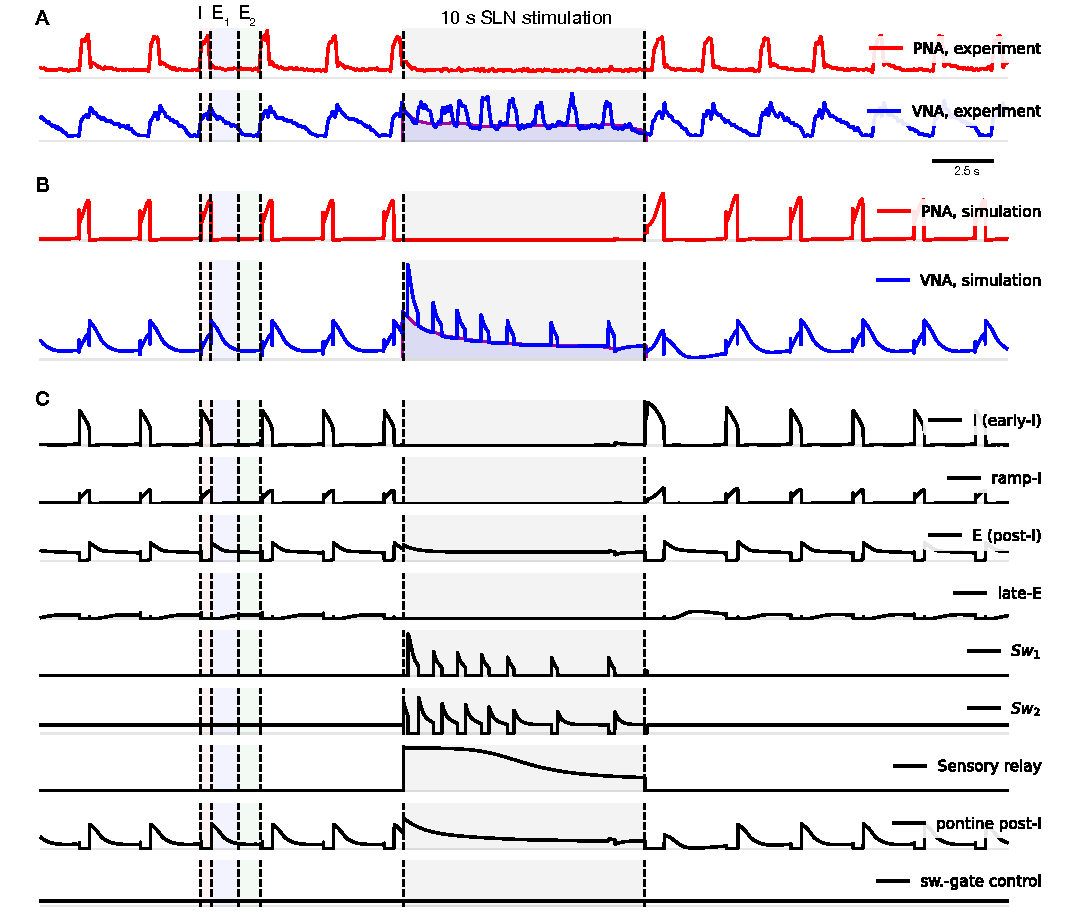
\includegraphics[width=1.0\textwidth]{Figures/4_swallowing_and_eupneic_breathing.pdf}
 \end{center}
 \caption{\textbf{Comparison of the model output with the original recordings.}
 The model reproduces eupneic breathing pattern with distinguished three phases. The comparison of experimental (\textbf{A}) and simulated recordings (\textbf{B}) from the activities of the phrenic and vagus nerve activities (PNA, VNA) is presented on the four upper traces. (\textbf{C}) The rest of the traces show the activities of the individual simulated neuronal populations. 
 The model also qualitatively reproduces the effects of the superior laryngeal nerve (SLN) stimulation. The oscillations in R-CPG are silenced by the `Sensory Relay' neurons, and the respiratory rhythm is locked in the postinspiratory phase. Meanwhile, the sensory neurons activate the Sw-CPG, and the network produces swallowing-related oscillations, with the progressively decreasing frequency of swallows. During the sequential swallowing, the phasically active pontine `post-I' population of neurons in the dorsolateral pons is responsible for the swallowing-related glottal closure. In the model, we assume that the phrenic nerve activity is driven solely by the `Ramp-I' neurons, whereas the vagus nerve activity is simulated as a combination of `Pontine Post-I', `Ramp-I' and `$\text{Sw}_1$' populations with coefficients 0.75, 0.9 and 0.6 correspondingly.
}\label{fig: swallowing_and_eupneic_breathing}
\end{figure}

\begin{figure}
 \begin{center}
 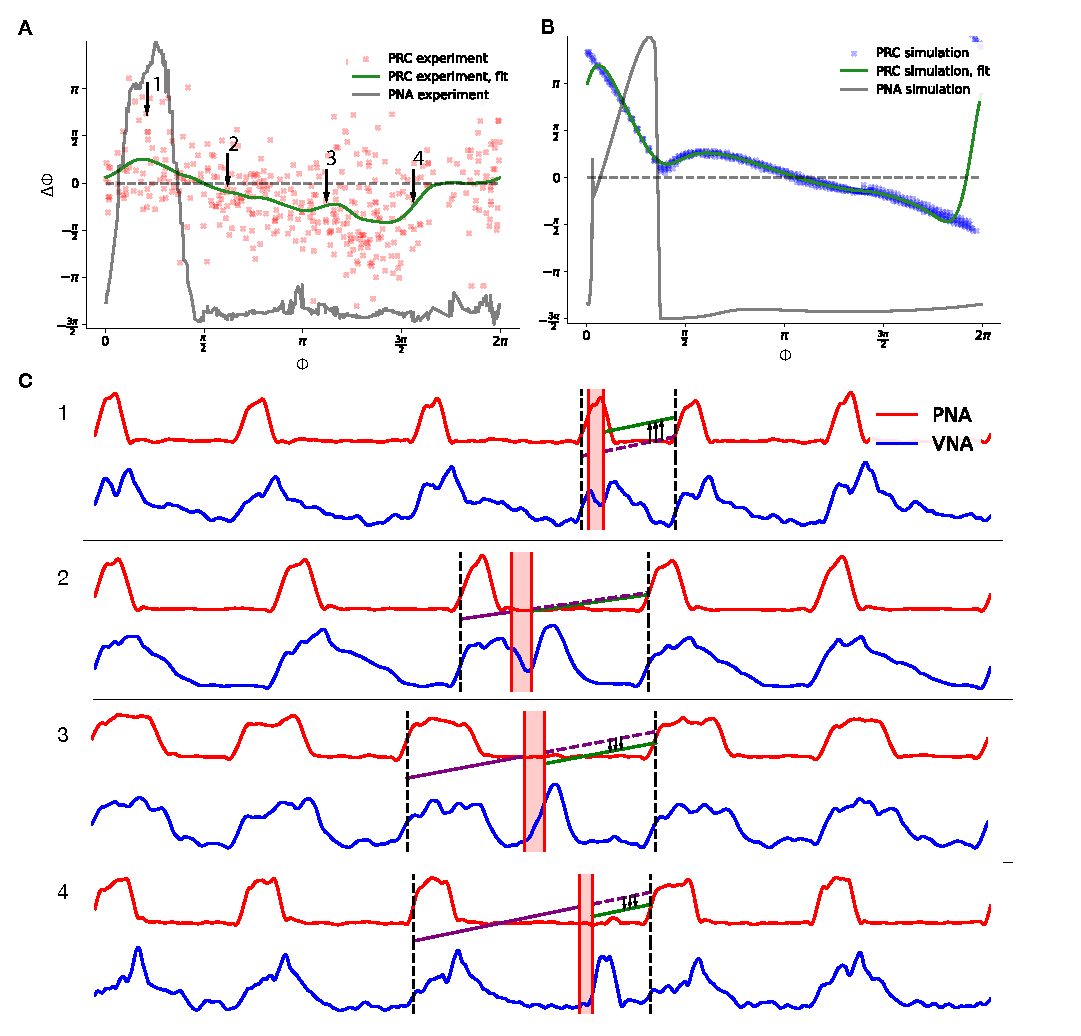
\includegraphics[width=1.0\textwidth]{Figures/5_comparison_PRC.pdf}
 \end{center}
 \caption{
 Short stimulation of the superior laryngeal nerve elicits a single swallow, which interferes with the respiratory cycle as characterized by a phase response curve (PRC). The PRC is estimated from the experimental data (\textbf{A}, 250~ms stimulation, red crosses and red curve) is qualitatively matched by the PRC of the simulated model (\textbf{B}, 100~ms stimulation, blue circles, blue curve). Experimentally acquired phrenic nerve activity associated with the data-points of the experimental PRC (\textbf{C}).
 Both PRCs indicate the delay of the next inspiration when the stimulation is applied during the late expiration (the region with the negative phase shift). The experimental and simulated PRCs both capture the effects of a short SLN stimulus application during the inspiration: termination of the inspiration and the new burst of inspiratory activity shortly after (positive-phase-shift regions in A, B).
 The phase of oscillations was estimated by linear fit $\omega t + c$ before (purple line) and after (green line) the stimulus onset; the phase shift $\Delta \Phi$ was quantified through measuring the discrepancy in free coefficients of a linear fit (see Sec. Data analysis).
}\label{fig: PRC_comparison}
\end{figure}
 % (\textbf{A}) Example Phrenic nerve activity (PNA) recording shows that a brief (250 ms) SLN stimulation (red shading) shifts the respiratory rhythm phase. The resulting phase shift was extracted by fitting the phase by a line with the same slope before and after the stimulation.

\begin{figure}
 \begin{center}
 
\includegraphics[width=1.0\textwidth]{Figures/6_PIR_mechanism_stability_analysis.pdf}
 \end{center}
 \caption{A short 100~ms stimulation of the superior laryngeal nerve (depicted by grey shadings) elicits a response in the Sw-CPG. Here we isolate the swallowing CPG and provided an external stimulus from the `Sensory Relay' neurons to study the mechanisms underlying the generation of the single swallow in the swallowing half-center oscillator. Sub-figures (\textbf{A}) and (\textbf{C}) depict the traces of the half-center oscillator: the simulated membrane potential variables $v_1$, $v_2$ and adaptation variables $m_1$ and $m_1$; index 1 denotes the premotor swallowing neurons. The swallowing premotor neurons are strongly inhibited in the absence of the external input, however, are readily excitable. 
 The phase space analysis of the ongoing dynamics is depicted in the subfigures (\textbf{B}) and (\textbf{D}). Since the $v$-variables (fast subsystem) evolve on a much faster time scale than the m variables (slow subsystem), for each pair of the m-variables the equilibria points for the v-variables of the dynamics were calculated. Taken altogether, these fixed points form a cusp-like equilibrium surface of the fast subsystem. The slow subsystem governs the evolution of the whole system once the system reaches the stable submanifolds of the equilibrium surface. The stable submanifold of the surface is denoted by the navy blue color, versus sky blue for the unstable equilibria. 
 In both scenarios (\textbf{B}) and (\textbf{D}), the equilibria surface is the same. The difference between the two scenarios lays in the values of the stimulus supply to each population of the half-center oscillator: in the first case, the stimulation strengths are $(0.12, 0.07)$ to `$\text{Sw}_1$' (premotor) and `$\text{Sw}_2$' populations correspondingly, whereas in the second scenario the stimulation strengths are $(0.19, 0.07)$, thereby in the latter case the `$\text{Sw}_1$' neuron inhibits `$\text{Sw}_2$' during the stimulus, however, returns to quiescence after the transient burst of activity.
}\label{fig: PIR_mechanism}
\end{figure}

\begin{figure}
 \begin{center}
 
\includegraphics[width=1.0\textwidth]{Figures/7_swallowing_and_apneustic_breathing.pdf}
 \end{center}
 \caption{\textbf{Simulated transection of pons influencing the breathing-swallowing coordination.} 
 (\textbf{A}) The lesioned circuit with all the pontine populations and drives removed. (\textbf{B}) The simulated phrenic and vagus nerve activity (PNA, VNA) of the intact model are compared to the same (\textbf{C}) outputs of the lesioned network. (\textbf{D}) The simulated average membrane potential traces of neuronal populations of the lesioned circuit. The network demonstrates an apneustic two-phased regime, lacking postinspiratory activity in its output. The 10~s sensory stimulation triggers the sequential swallowing response, although the concomitant swallowing-related glottal closure is absent. The simulated pontine lesion has also alleviated inhibition of premotor swallowing neurons $\text{Sw}_1$, and the latter become active throughout the respiration, resembling the spontaneous activity observed in the experiments. 
}\label{fig: eupn_vs_apn}
\end{figure}

\begin{figure}
 \begin{center}
 
\includegraphics[width=0.9\textwidth]{Figures/8_pathological_behavior.pdf}
 \end{center}
 \caption{\textbf{Pathological interactions between breathing and swallowing networks}
 (\textbf{A}) Simulated healthy swallowing response.
 (\textbf{B}) Simulated pathological activity in the phrenic nerve caused by the weakened sensory inhibition of the inspiratory neurons, both `I' and `Ramp-I'.
 In the simulation, the strength of the sensory inhibition $W_{\text{Sens. Relay} \to \text{I}}$ and $W_{\text{Sens. Relay} \to \text{Ramp-I}}$ were both set to $-0.22$ (vs. $-0.4$ in the intact network). The simulated inspiratory breakthroughs are biphasic, since the inspiratory neuronal populations are inhibited by the `$\text{Sw}_1$' group, and the latter becomes active during the inspiratory breakthrough transiently inhibiting the pathological inspiration. 
 (\textbf{C}) Weakened and delayed swallowing response in the model of the R-CPG-Sw-CPG network reflected in the response of vagus nerves to the long SLN stimulation. For the simulation, the parameter $W_{\text{Sens. Relay} \to \text{Sw}_1} = 0.052$ (vs. $0.12$ in the intact network). The corresponding traces of the normal swallowing response are shown in the panel for comparison;
 PNA -- phrenic nerve activity; VNA -- Vagus nerve activity.
 }\label{fig: pathological_behavior}
\end{figure}


\begin{figure}
 \begin{center}
 
\includegraphics[width=0.97\textwidth]{Figures/9_varying_params_sw_neurons.pdf}
 \end{center}
 \caption{\textbf{Control of the swallowing: variation of the parameters of the Sw-CPG.} To acquire each point on a graph, we simulated the network applying a long stimulation of `Sensory Relay' (Amplitude $A=0.45$, duration $T = 10$~s) to quantify the sequential swallowing response, and a short stimulation ($A=0.45$, $T=100$~ms) -- to illuminate the presence of the evoked solitary after-stimulus swallow (depicted by $*$ on the panel with simulated phrenic (PNA) and vagus (VNA) nerve responses). The default value of the parameter is depicted by a grey solid line. Blue-shaded regions highlights regions where spontaneous swallows occur. See text for details.
 }\label{fig: sensitivity_analysis}
\end{figure}


\section{Tables}

% --- in the body ---
\begin{center}
\begin{tabular}{l|c|c|c|c}
\hline
Node 1 $\to$ Node 2 & Model 1 & Model 2 & Model 3 & Model 4 \\ \hline
SR $\to$ Sw$_1$ & +0.12 & +0.12 & +0.12 & +0.12\\ 
SR $\to$ Sw$_2$ & +0.07 & +0.07 & +0.07 & +0.07\\ 
SR $\to$ Pont. Post-I & 0.00 & +0.03 & +0.03 & +0.03\\ 
SR $\to$ I & -0.40 & -0.40 & -0.40 & -0.40\\ 
SR $\to$ Late-E & 0.00 & 0.00 & -0.40 & -0.40\\ 
SR $\to$ Ramp-I & 0.00 & 0.00 & 0.00 & -0.40\\ 
Sw$_1 \to$ Sw$_2$ & -0.90 & -0.90 & -0.90 & -0.90\\ 
Sw$_1 \to$ I & -0.80 & -0.80 & -0.80 & -0.80\\
Sw$_1 \to$ Ramp-I & 0.00 & 0.00 & 0.00 & -0.80\\
Sw$_1 \to$ Late-E & 0.00 & 0.00 & -0.20 & -0.20\\
Sw$_2 \to$ Sw$_1$ & -0.65 & -0.65 & -0.65 & -0.65\\
I $\to$ E (Post-I) & -0.30 & -0.30 & -0.20 & -0.20\\
I $\to$ Late-E & 0.00 & 0.00 & -1.00 & -1.00\\
I $\to$ Sw$_1$ & -0.01 & -0.01 & -0.01 & -0.01\\
I $\to$ Pont. Post-I & 0.00 & -0.35 & -0.35 & -0.35\\
I $\to$ Ramp-I & 0.00 & 0.00 & 0.00 & -0.22\\
E (Post-I) $\to$ Insp & -0.70 & -0.70 & -0.50 & -0.50\\
E (Post-I) $\to$ Ramp-I & 0.00 & 0.00 & 0.00 & -1.00\\
E (Post-I) $\to$ Late-E & 0.00 & 0.00 & -1.30 & -1.30\\
E (Post-I) $\to$ Pont. Post-I & 0.00 & +0.03 & +0.03 & +0.03\\
Late-E $\to$ E (Post-I) & 0.00 & 0.00 & -0.01 & -0.01\\
Late-E $\to$ Pont. Post-I & 0.00 & 0.00 & -0.65 & -0.65\\
Late-E $\to$ I & 0.00 & 0.00 & -0.70 & -0.70\\
Late-E $\to$ Ramp-I & 0.00 & 0.00 & 0.00 & -0.75\\
Pont. Post-I $\to$ E (Post-I) & 0.00 & +0.03 & +0.03 & +0.03\\
Sw. gate $\to$ Sw$_1$ & 0.00 & -0.15 & -0.15 & -0.15\\
Sw$_1 \to$ VN & --- & --- & --- & +0.60\\
Ramp-I $\to$ VN & --- & --- & --- & +0.90\\
Post-I $\to$ VN & --- & --- & --- & +0.20\\
Pont. Post-I $\to$ VN & --- & --- & --- & +0.55\\
Ramp-I $\to$ PN & --- & --- & --- & +1.00\\ \hline
\end{tabular}
\captionof{table}{Connectivity description. SR---Sensory Relay; VN---Vagus nerve; PN---Phrenic nerve}\label{tbl: connectivity_params}
\end{center}


%==================================================
\begin{center}

\begin{tabular}{lc}\hline
Drive & Value\\ \hline
Chemo drive $\to$ I & 0.30\\
Chemo drive $\to$ Ramp-I & 0.30\\
Chemo drive $\to$ Late-E & 0.45\\
Chemo drive $\to$ Pont. Post-I & 0.05\\
Arousal drive $\to$ Sw$_1$ & \textbf{0.19}$^{*}$\\
Arousal drive $\to$ Sw$_2$ & 0.35\\
Arousal drive $\to$ Sw. gate & 0.25\\
Pontine drive $\to$ E (Post-I) & 0.35\\
Pontine drive $\to$ I & 0.05\\
Pontine drive $\to$ Ramp-I & 0.05\\ \hline
\end{tabular}
\footnotesize 
\end{center}
\captionof{table}{Excitatory drives to populations. $^{*}$For Model 1, the arousal drive to Sw$_1$ is 0.16.}\label{tbl: drives}

% %==================================================
\begin{center}
\begin{tabular}{lc}\hline
Population & $\tau_m$ (ms) \\ \hline
I & 5000 \\
Ramp-I & 5000 \\
E (Post-I) & 5000 \\
Late-E & 5000 \\
Sw$_1$ & 1500 \\
Sw$_2$ & 1500 \\
Sensory Relay & 17500 \\
Pont. Post-I & 10000 \\
Sw. gate & 5000 \\ \hline
\end{tabular}
\captionof{table}{Intrinsic parameters. For all populations: $\alpha=1$, $b=0.2$, $\tau_v=2$~ms, $\lambda=30$.}\label{tbl: intrinsic_params}
\end{center}
% \backmatter
% \bmhead{Supplementary information}

% If your article has accompanying supplementary file/s please state so here. 

% Authors reporting data from electrophoretic gels and blots should supply the full unprocessed scans for key as part of their Supplementary information. This may be requested by the editorial team/s if it is missing.

% Please refer to Journal-level guidance for any specific requirements.

\section*{Author contributions}
M.D., R.R.D., P.T., and J.H.M. formulated the research question and contributed to the study design. R.R.D. collected and curated the experimental data. P.T. developed the code-base, conducted the simulations, analyzed simulated data and processed experimental data. P.T., M.D., and R.R.D. jointly wrote the manuscript.

\section*{Acknowledgements}
We acknowledge that this work was conducted on the traditional land of the Wurundjeri people of the Kulin nation. We pay our respect to their elders past, present and emerging.

\section*{Funding Declaration}
This work was supported by the National Health and Medical Research Council of Australia (APP1165529, awarded to M.D.). The funder had no role in study design, data collection, analysis, or manuscript preparation.

\section*{Data availability}
The experimental recordings of phrenic and vagal nerve activity during short and long SLN stimulation are publicly available on Zenodo at:
\href{https://zenodo.org/records/18750367}{https://doi.org/10.5281/zenodo.18750367}.

\section*{Code availability}
The code for modeling, PRC extraction, and experimental data processing is available on GitHub at \href{https://github.com/ptolmachev/SimplifiedModel_rCPG_swCPG_interaction}{https://github.com/ptolmachev/SimplifiedModel\_rCPG\_swCPG\_interaction}.

% Please refer to Journal-level guidance for any specific requirements.


% Some journals require declarations to be submitted in a standardised format. Please check the Instructions for Authors of the journal to which you are submitting to see if you need to complete this section. If yes, your manuscript must contain the following sections under the heading `Declarations':

% \begin{itemize}
% \item Funding
% \item Conflict of interest/Competing interests (check journal-specific guidelines for which heading to use)
% \item Ethics approval and consent to participate
% \item Consent for publication
% \item Data availability 
% \item Code availability 
% \item Materials availability
% \item Author contribution
% \end{itemize}

% \noindent
% If any of the sections are not relevant to your manuscript, please include the heading and write `Not applicable' for that section. 

% %%===================================================%%
% %% For presentation purpose, we have included %%
% %% \bigskip command. Please ignore this. %%
% %%===================================================%%
% \bigskip
% \begin{flushleft}%
% Editorial Policies for:

% \bigskip\noindent
% Springer journals and proceedings: \url{https://www.springer.com/gp/editorial-policies}

% \bigskip\noindent
% Nature Portfolio journals: \url{https://www.nature.com/nature-research/editorial-policies}

% \bigskip\noindent
% \textit{Scientific Reports}: \url{https://www.nature.com/srep/journal-policies/editorial-policies}

% \bigskip\noindent
% BMC journals: \url{https://www.biomedcentral.com/getpublished/editorial-policies}
% \end{flushleft}

% \begin{appendices}

% \section{Section title of first appendix}\label{secA1}

% An appendix contains supplementary information that is not an essential part of the text itself but which may be helpful in providing a more comprehensive understanding of the research problem or it is information that is too cumbersome to be included in the body of the paper.
%%=============================================%%
%% For submissions to Nature Portfolio Journals %%
%% please use the heading ``Extended Data''. %%
%%=============================================%%
%%=============================================================%%
%% Sample for another appendix section			 %%
%%=============================================================%%
%% \section{Example of another appendix section}\label{secA2}%
%% Appendices may be used for helpful, supporting or essential material that would otherwise 
%% clutter, break up or be distracting to the text. Appendices can consist of sections, figures, 
%% tables and equations etc.
% \end{appendices}
%%===========================================================================================%%
%% If you are submitting to one of the Nature Portfolio journals, using the eJP submission %%
%% system, please include the references within the manuscript file itself. You may do this %%
%% by copying the reference list from your .bbl file, paste it into the main manuscript .tex %%
%% file, and delete the associated \verb+\bibliography+ commands. %%
%%===========================================================================================%%
\bibliography{bibliography}% common bib file
%% if required, the content of .bbl file can be included here once bbl is generated
% \input sn-article.bbl

\end{document}
